%!TEX root = ../colloquium.tex

\begin{frame}[plain,noframenumbering]
	\centering
	\vspace*{2.6cm}
	\Huge \colorit{Part I}
	\vskip 20pt
	\Large Persistent homology
\end{frame}

\begin{frame}{Points clouds and multi-scale approximation}
	\pause
	Data sets are often encountered as point clouds in $\R^n$

	\pause
	\begin{center}
		\includegraphics[scale=.35]{aux/point_cloud_cropped}
	\end{center}

	\pause\vskip-3pt
	Underlying probability dist. concentrated on a subspace.
	\pause
	\pcolor{What is its shape?}

	\pause\medskip
	Given a scale $t \in \R_{\geq 0}$ construct a graph $X_t$
	\begin{center}
		\vskip-3pt
		\includegraphics[scale=.09]{aux/network_cropped}
	\end{center}
	\vskip-6pt
	approximating it.
	\pause
	\pcolor{What is the ``right" scale?}
\end{frame}

\begin{frame}{Points clouds and multi-scale approximation}
	\pause
	Consider \pcolor{all} scales and obtain a family of nested graphs
	\[
	X_{t_0} \subset X_{t_1} \subset\dots\subset X_{t_n}
	\]
	with $t_i$ a value where the the graph changes.

	\medskip\pause
	From these we can track connected components of $X_t$ as $t$ varies.

	\medskip\pause
	\pcolor{Example}:

	\begin{center}
		\includegraphics[scale=.25]{aux/2Dcloud_cropped.pdf}
		\pause\qquad
		\includegraphics[scale=.313]{aux/2Dbarcode_cropped.pdf}
	\end{center}

	\medskip\pause
	Longer bars correspond to features that \pcolor{persist}.
\end{frame}

\begin{frame}{Points clouds and multi-scale approximation}
	\pause
	A \pcolor{simplicial complex} is a generalization of a graph
	\begin{center}
		\includegraphics[scale=.1]{aux/torus_triangulated}
	\end{center}
	with higher dimensional ``edges" termed \pcolor{simplices}.

	\medskip\pause
	Given a point cloud, the graph $X_t$ had an edge $[v,w]$ between $v$ and $w$ iff
	\[
	distance(v,w) \leq t.
	\]
	\pause
	The simplicial complex $X_t$ has an $n$-simplex $[v_0,v_1,\dots,v_n]$ if
	\[
	\forall i,j, \quad distance(v_i,v_j) \leq t.
	\vspace*{-5pt}
	\]
	\vspace*{-5pt}\pause
	Obtain \pcolor{filtered simplicial complex}
	\[
	X_{t_0} \subset X_{t_1} \subset\dots\subset X_{t_n}
	\]
\end{frame}

\begin{frame}{Robust/stable invariants}
	\pause
	We want invariants of the underlying space/shape not of the simplicial complex approximating it.

	\medskip
	\colorit{E.g.} Alternative point cloud samples should give the same or ``similar" invariants.

	\pause\medskip
	\colorit{Bad ideas}: count number of simplices, measure incidence angles, record volumes,...

	\medskip
	All of these depend on the simplicial complex.

	\pause\medskip
	\colorit{Basic example}: (Euler characteristic)
	\[
	\chi = \# vertices - \# edges + \dots + (-1)^n \#(n\text{-}simplices).
	\]
\end{frame}

\begin{frame}{Finer features: Homology}
	\pause
	Given a simplicial complex $X$
	\begin{center}
		\includegraphics[scale=.1]{aux/torus_triangulated}
	\end{center}
	the \pcolor{homology} construction produces $\forall d \in \N$ a vector space $H_d(X)$ whose dimension $\beta_d(X)$ counts the ``$d$-dim'l components'' or ``$d$-cavities" of $X$.

	\pause\medskip
	\pcolor{Remark} $\beta_0$ is the usual number of connected component.

	\pause\smallskip
	\pcolor{Remark} $\beta_0 - \beta_1 + \dots + (-1)^n \beta_n$ is $\chi$.

	\pause\medskip
	\pcolor{Example} if $T$ is the above space
	\[
	\beta_0(T) = 1, \quad \beta_1(T) = 2, \quad \beta_2(T) = 1, \quad \beta_i(T) = 0.
	\]
	It is connected, has two independent loops, \\
	and one 2-dimensional cavity.
\end{frame}

\begin{frame}{Persistence homology}
	\pause
	Applying homology to the multi-scale approximation\vspace*{-5pt}
	\[
	X_{0} \subset X_{1} \subset\dots\subset X_{n}
	\vspace*{-5pt}
	\]
	gives a family of vector spaces and linear maps\vspace*{-5pt}
	\[
	H_d(X_0) \to H_d(X_1) \to\dots\to H_d(X_n).
	\]
	\pause
	The way their dimensions $\beta_d$ ``fit together" defines the $d^\th$ \pcolor{barcode}.

	\pause\smallskip
	\begin{center}
		\includegraphics[scale=.7]{aux/vietoris-rips}
		\includegraphics[scale=.6]{aux/betti}
	\end{center}

	\begin{minipage}{.5\textwidth}
		\pause
		Abstractly, a \pcolor{barcode} is a collection of pairs $(a,b) \in \R^2$ with multiplicity.
	\end{minipage}%
	\hspace*{1cm}
	\begin{minipage}{.3\textwidth}
		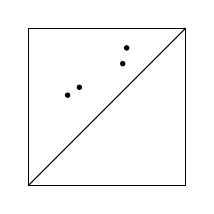
\begin{tikzpicture}[scale=.5]
			% Draw square
			\draw (0,0) rectangle (4,4);
			% Draw diagonal
			\draw (0,0) -- (4,4);
			% Draw points above the diagonal
			\fill (1,2.3) circle (2pt);
			\fill (1.3,2.5) circle (2pt);
			\fill (2.4,3.1) circle (2pt);
			\fill (2.5,3.5) circle (2pt);
		\end{tikzpicture}
	\end{minipage}
\end{frame}

\begin{frame}{Why are barcodes useful?}
	\pause\smallskip
	1. \colorit{Stability}: The passage from point clouds to barcodes preserves distances.

	\pause\smallskip
	\begin{minipage}{.6\textwidth}
		Point cloud distance is \pcolor{Gromov--Hausdorff}:
	\end{minipage}
	\hspace*{10pt}
	\begin{minipage}{.3\textwidth}
		\begin{tikzpicture}[scale=.7]
			\draw[dashed, red] (-1.5,1.5) -- (0,0);
			\draw[dashed, blue] (1,2) -- (.7,.7);
			% Draw blue points
			\fill[blue] (0,0) circle (2pt);
			\fill[blue] (1.3,1.5) circle (2pt);
			\fill[blue] (1,2) circle (2pt);
			% Draw red points
			\fill[red] (.7,.7) circle (2pt);
			\fill[red] (-1.5,1.5) circle (2pt);
		\end{tikzpicture}
	\end{minipage}

	\pause\smallskip
	\begin{minipage}{.5\textwidth}
		Point cloud distance is \pcolor{Bottleneck}:
	\end{minipage}
	\hspace*{0pt}
	\begin{minipage}{.3\textwidth}
		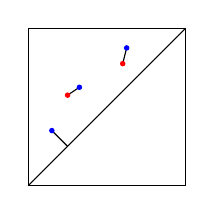
\begin{tikzpicture}[scale=.5]
			% Draw square
			\draw (0,0) rectangle (4,4);
			% Draw diagonal
			\draw (0,0) -- (4,4);
			% Draw edges
			\draw[] (1,2.3) -- (1.3,2.5);
			\draw[] (2.4,3.1) -- (2.5,3.5);
			\draw[] (.6,1.4) -- (1,1);

			% Draw points above the diagonal
			% Adjust the coordinates as needed to position your points
			\fill[red] (1,2.3) circle (2pt);
			\fill[blue] (1.3,2.5) circle (2pt);
			\fill[red] (2.4,3.1) circle (2pt);
			\fill[blue] (2.5,3.5) circle (2pt);
			\fill[blue] (.6,1.4) circle (2pt);
		\end{tikzpicture}
	\end{minipage}

	\pause\bigskip
	\[
	d_{GH}(X,Y) \leq d_{b}(\cB_X, \cB_Y)
	\]

	\pause\medskip
	2. \colorit{Computability}: Based on matrix reduction algorithms, it complexity is
	\[
	\sim O(\# \text{simplices}^3).
	\]
\end{frame}

\begin{frame}{Exemplar - Nanoporous materials (Lee et al.)}
	\pause
	\textcolor{pblue}{Comparing geometries} \\
	directly, impossible, \\
	over 3M structures.

	\begin{textblock*}{4cm}(5.4cm,1.5cm)
		\includegraphics[scale=.28]{aux/real_material}
	\end{textblock*}

	\pause\vspace*{2cm}
	\textcolor{pblue}{Comparing Barcodes} \\
	is done fast \\
	and faithfully \\
	by stability.

	\vspace*{-2.3cm}\hspace*{3.8cm}
	\includegraphics[scale=.6]{aux/nanoporous}
\end{frame}

\begin{frame}{Where to find these tools? \texttt{giotto-tda}}
	\pause
	Integration of persistence algorithms into \texttt{scikit-learn}.
	\vskip 10pt
	\includegraphics[scale=.31]{aux/giotto}
\end{frame}